% Created 2020-04-07 Tue 20:17
\documentclass[9pt, b5paper]{article}
\usepackage{fontspec}
\usepackage{graphicx}
\usepackage{xcolor}
\usepackage[slantfont,boldfont]{xeCJK}
\setCJKmainfont[BoldFont = Heiti SC, ItalicFont = STFangsong]{STSong}
\setCJKsansfont{STHeiti}
\setCJKmonofont{STFangsong}
\usepackage{multirow}
\usepackage{multicol}
\usepackage{float}
\usepackage{textcomp}
\usepackage{geometry}
\geometry{left=1.2cm,right=1.2cm,top=1.5cm,bottom=1.0cm}
\usepackage{algorithm}
\usepackage{algorithmic}
\usepackage{latexsym}
\usepackage{natbib}
\usepackage{listings}
\usepackage{minted}
\usepackage[xetex,colorlinks=true,CJKbookmarks=true,linkcolor=blue,urlcolor=blue,menucolor=blue]{hyperref}
\author{deepwaterooo}
\date{\today}
\title{Android Developer Interview Questions}
\hypersetup{
  pdfkeywords={},
  pdfsubject={},
  pdfcreator={Emacs 26.3 (Org mode 8.2.7c)}}
\begin{document}

\maketitle
\tableofcontents


\section{Important and frequently asked Android developer interview questions}
\label{sec-1}
\begin{itemize}
\item \url{https://www.educba.com/android-developer-interview-questions/}
\item \url{https://www.educba.com/android-interview-questions/}
\end{itemize}
\subsection{Android}
\label{sec-1-1}
\subsubsection{Explain Platform Architecture of android? And what is Google Android SDK?}
\label{sec-1-1-1}
\begin{itemize}
\item Android is an open source, LINUX based software pack. It mainly comprises of 
\begin{itemize}
\item Linux Kernel
\item Hardware Abstraction Layer (HAL)
\item Native libraries, Android Runtime
\item Java API
\item System Apps
\end{itemize}
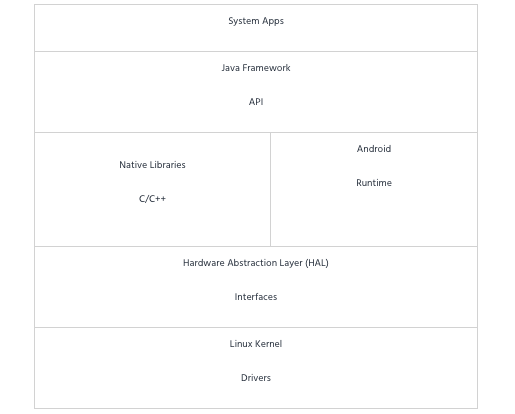
\includegraphics[width=.9\linewidth]{./pic/androidArchtecture.png}
\item Talking from bottom to top
\item \textbf{Linux Kernel}:
\begin{itemize}
\item The base layer of an application that directly interfaces with the device hardware.
\item the Linux kernel provides drivers for connecting to hardware.
\item The driver's list contains – Audio, Binder, Display, Keypad, Bluetooth, Camera, USB, Wi-Fi and power management.
\end{itemize}
\item \textbf{Hardware Abstraction Layer (HAL)}:
\begin{itemize}
\item The Hardware Abstraction Layer (HAL) provides a standard that interacts with Kernel drivers to access these hardware features to the users.
\end{itemize}
\item \textbf{Android Runtime}:
\begin{itemize}
\item ART (Android Runtime) is there to help when multiple virtual machines (VM's) are run on low memory devices with the execution of DEX files.
\item The Dalvik Virtual Machine is in the same level as the Native Libraries and allows every Android app to run its own processes.
\end{itemize}
\item \textbf{Native libraries}:
\begin{itemize}
\item Native C or C++ is needed to build the native code.
\item \emph{a set of open-source libraries, including the SQLite database, libc, and the WebKit browser engine. ???}
\end{itemize}
\item \textbf{Java API}:
\begin{itemize}
\item Android provides Java API's to use functionalities of native libraries to the apps.
\item Java API forms the building blocks on a need to create Android apps by providing the components and services.
\item This level provides higher-level services in the form of Java classes to applications on the device. The key services to know are the Activity Manager, Content Providers, Resource Manager, Notifications Manager, and the View System.
\end{itemize}
\item \textbf{System Apps}:
\begin{itemize}
\item Android comes with a set of core apps for emails, SMS messaging, calendars, internet browsing, contacts and more.
\end{itemize}
\item \textbf{Google SDK} is \emph{a development toolkit} that is used by developers to write programs for mobile devices. It provides a graphical user interface simulating Android driven environment and enabling the developer to test and debug their codes.
\end{itemize}

\subsubsection{Can you describe the core building blocks of an Android application?}
\label{sec-1-1-2}
\begin{itemize}
\item This top-level question is a great way to warm up the developer and get a feel for how well they understand the basics of building an Android app from scratch. The basic components are as follows:
\begin{itemize}
\item \textbf{Activity}: An activity is a subclass of the \textbf{ContextThemeWrapper} class. Since almost all activities interact directly with the user, it is often helpful to think of an activity as the screen for a particular action, such as logging in or taking a picture.
\item \textbf{View}: The view is everything you can see on the screen of the app—think of the individual UI elements like buttons, labels, and text fields.
\item \textbf{Intent}: The main purpose of intent is to invoke individual components. Common uses include starting the service, launching activities, displaying a list of contacts, dialing a phone number, or displaying a web page.
\item \textbf{Service}: A service is a background process that can either be local or remote. 
\begin{itemize}
\item \textbf{Local services} may be accessed from within the application
\item while \textbf{remote services} are intended to be used by other applications running on the same device.
\end{itemize}
\item \textbf{Content Provider}: Content providers share data between applications.
\item \textbf{Fragment}: Fragments are best thought of as parts of an activity—you can display more than one fragment on the screen at the same time.
\item \textbf{Android Manifest.xml}: The AndroidManifest.xml file provides essential information about your app required for it to run on the Android operating system. All Android apps have this file in their root directory.
\end{itemize}
\end{itemize}
\subsubsection{Briefly explain the components/requirements for any Android development projects?}
\label{sec-1-1-3}
\begin{itemize}
\item This is the most popular Android developer Interview Questions asked in an interview. The below-listed components are needful for successful completion:
\begin{itemize}
\item \textbf{Build}: contains the build output.
\item \textbf{Src}: holds the code and resource file.
\item \textbf{Res}: holds the bitmap images, UI, XML layouts.
\item \textbf{Assets}: holds the file which can be combined into a .apk file.
\item \textbf{Manifest}: holds the XML file.
\end{itemize}
\end{itemize}
\subsubsection{Explain in brief the files and folder which are created when an Android project is created.}
\label{sec-1-1-4}
\begin{itemize}
\item The new project should have following files in the package in eclipse.
\begin{itemize}
\item \textbf{src} This file contains java source files for the newly created project. The code for the application is to be written in this file. It should be made available under the name of a project.
\item \textbf{Assets} This is a folder which will contain all information regarding HTML files, text files, and databases.
\item \textbf{gen} This folder must have the R.java file. It is a file generated by the compiler and it references the resources that are found in the project. This file should not be modified as it is generated by the compiler.
\item \textbf{Android library} This folder contains an android.jar file which has all libraries needed for creating an Android application.
\item \textbf{bin} It contains the .apk file that is created by ADT during the code build process. This file is the application binary file. When a developer runs his code this file has everything required to run a code.
\item \textbf{res} This is a folder that contains all resource files used by the application. It has subfolders like drawable, menu, layout, and values etc.
\end{itemize}
\end{itemize}
\subsubsection{What are the important items in Android and explain the importance of XML based layouts?}
\label{sec-1-1-5}
\begin{itemize}
\item The must required items in an Android project when a project is created are as below:
\begin{itemize}
\item Androidmanifest.xml
\item Build.xml
\item bin
\item src
\item res
\item assets
\end{itemize}
\item Here we have two XML files which help in providing a consistent layout. It helps in giving the developer a standard graphical definition format. Usually, all layout details are placed in these XML files and the other items are placed in source files.
\end{itemize}
\subsubsection{What is DDMS? Describe some of its capabilities.}
\label{sec-1-1-6}
\begin{itemize}
\item DDMS is short for Dalvik Debug Monitor Server. It ships natively with Android and contains a number of useful debugging features including: 
\begin{itemize}
\item port-forwarding services       端口转发服务
\item screen capture                 屏幕截图
\item thread and heap information    线程和堆信息
\item network traffic tracking       网络跟踪
\item incoming call/SMS spoofing     来电和短信监听
\item simulating network state, speed, and latency 模拟网络状态,速度和延迟
\item location data spoofing                       位置数据监听
\end{itemize}
\end{itemize}
\begin{center}
\begin{tabular}{ll}
\hline
port-forwarding services & 端口转发服务\\
screen capture & 屏幕截图\\
thread and heap information & 线程和堆信息\\
network traffic tracking & 网络跟踪\\
incoming call/SMS spoofing & 来电和短信监听\\
simulating network state, speed, and latency & 模拟网络状态,速度和延迟\\
location data spoofing & 位置数据监听\\
\hline
\end{tabular}
\end{center}

\subsubsection{Why did you become an Android developer? What are some of the advantages of the Android platform?}
\label{sec-1-1-7}
\begin{itemize}
\item You want a developer who really knows how to play to the strengths of your chosen platform. Some key advantages of Android are listed below for your convenience.
\begin{itemize}
\item \textbf{Open Source}: No licenses, no distribution or development fees.
\item \textbf{DVM (Dalvik Virtual Machine)}: DVM is a highly optimized virtual machine for mobile devices.
\item \textbf{Platform Diversity}: Since Android is open-source, it has been adopted by a wide range of manufacturers of mobile devices.
\item \textbf{Experience with Java}: Java is the language of choice for Android app development. Those who already have years of experience in Java will feel right at home developing for Android.
\end{itemize}
\end{itemize}
\subsubsection{What is difference between Serializable and Parcelable? Which is best approach in Android?}
\label{sec-1-1-8}
\begin{itemize}
\item \textbf{Serializable} is a standard Java interface that's easy to integrate into your app, as it doesn't require any methods. You simply mark a class Serializable by implementing the interface, and Java will automatically serialize it in certain situations. Despite being easy to implement, Serializable uses the Java reflection API, which makes it a slow process that creates lots of temporary objects.
\item \textbf{Parcelable} is an Android specific interface where you implement the serialization yourself. It was created to be far more efficient than Serializable, and to get around some problems with the default Java serialization scheme. \textbf{Parcelable} is optimized for Android, so it's faster than Serializable. It's also fully customizable, so you can be explicit about the serialization process, which results in less garbage objects.
\item While the developer may acknowledge that implementing Parcelable does require more work, the performance benefits mean that they should advise using Parcelable over Serialization, wherever possible.
\end{itemize}
\subsubsection{Coin as many Android OS version that you remember?}
\label{sec-1-1-9}
\begin{center}
\begin{tabular}{ll}
\hline
VERSION & NAME\\
\hline
Android 8.0 & Oreo\\
Android 7.0 – 7.1.2 & Nougat\\
Android 6 – 6.0.1 & Marshmallow\\
Android 5 – 5.1.1 & Lollipop\\
Android 4.4 – 4.4.4 & KitKat\\
Android 4.1 – 4.3 & Jelly Bean\\
Android 4.0-4.0.4 & Ice Cream Sandwich\\
\hline
\end{tabular}
\end{center}

\subsection{Activity, Fragment, AsynTask, Lifecyles}
\label{sec-1-2}
\subsubsection{Explain the process to launch an activity on an application.}
\label{sec-1-2-1}
\begin{itemize}
\item To launch an activity developer needs to explicitly define intent. It specifies the activity that we wish to start. The following code will help you understand that activity which is sent in the second parameter in the new activity class. The first parameter is the Intent constructor in the current activity context.
\begin{minted}[linenos=true]{csharp}
Intent intent1= new Intent(this, SecondActivity.class);
startActivity(intent1);
\end{minted}

\item If the user wishes to start activity from a particular fragment then below can be tried: 
\begin{minted}[linenos=true]{csharp}
Intent intent1= new Intent(getActivity(), SecondActivity.class);
startActivity(intent1);
\end{minted}
\end{itemize}
\subsubsection{Can you explain the Android activity lifecycle?}
\label{sec-1-2-2}
\begin{itemize}
\item After a user navigates within the app, then the activity instances transit through different stages in their lifecycle.
\item These activity classes provide a number of actions called as "callbacks" that gives information of the changed states the system creates, resumes or stops while resuming the activity.
\item The activity life cycle has 4 states –
\begin{itemize}
\item \textbf{Active or running} – If the activity is in the foreground of the screen it is called as active.
\item \textbf{Paused} – If the activity has lost focus but is still visible (like in the case of dialog comes top), then it is reoffered as paused.
\item \textbf{Stopped} – If an activity is completely obscured by another activity, it's called as stopped. It still retains all states and the information of member components.
\item \textbf{Finish} – If an activity is paused or stopped, the system can drop the activity from memory by either asking it to finish or simply killing the process.
\end{itemize}
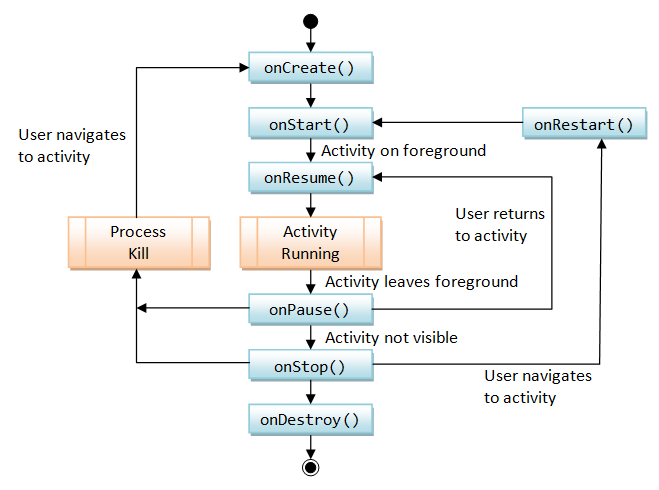
\includegraphics[width=.9\linewidth]{./pic/activityLifeCycle2.png}

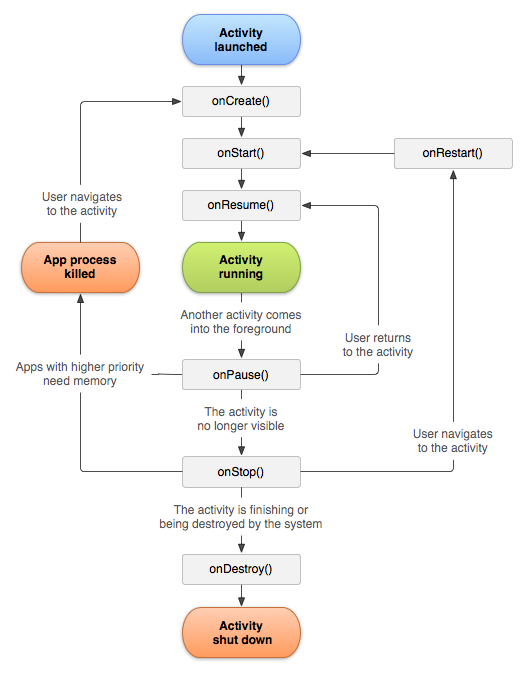
\includegraphics[width=.9\linewidth]{./pic/activityLifeCycle.png}
\end{itemize}
\subsubsection{What are the states of an activity?}
\label{sec-1-2-3}
\begin{itemize}
\item There are four states of an activity. They are:
\begin{itemize}
\item \textbf{Active}: When the activity is \textbf{active in the foreground}.
\item \textbf{Paused}: When activity is \textbf{in the background and still visible}.
\item \textbf{Stopped}: When activity is \textbf{not visible}.
\item \textbf{Destroyed}: When activity is \textbf{killed or terminated}.
\end{itemize}
\end{itemize}
\subsubsection{What are the seven lifecycle methods of Android activity and what is their purpose?}
\label{sec-1-2-4}
\begin{itemize}
\item The seven lifecycle methods of Android activity are 
\begin{itemize}
\item onCreate()
\item onStart()
\item onRestart()
\item onResume()
\item onPause()
\item onStop()
\item onDestroy()
\end{itemize}
\item Their purpose is to help structure your code around how you want an activity to perform throughout its lifecycle on the device.
\item For example, \textbf{onCreate()} is where you would perform your static setup, from creating views to binding data to lists. It is always immediately followed by \textbf{onStart()}, where the app will be made visible to the user.
\end{itemize}
\subsubsection{Write a quick script for launching a new activity within your application.}
\label{sec-1-2-5}
\begin{itemize}
\item The goal of this question is to quickly test their knowledge of explicit intent in launching an activity.
\item An explicit intent explicitly defines the activity the developer wishes to start. A possible solution has been produced below.
\begin{minted}[linenos=true]{java}
Intent myIntent = new Intent(this, MyNewActivity.class);
startActivity(myIntent);
\end{minted}
\end{itemize}
\subsubsection{onDestroy()}
\label{sec-1-2-6}
\begin{itemize}
\item \textbf{Question}: The last callback in the lifecycle of an activity is onDestroy(). The system calls this method on your activity as the final signal that your activity instance is being completely removed from the system memory. Usually, the system will call onPause() and onStop() before calling onDestroy(). Describe a scenario, though, where onPause() and onStop() would not be invoked.
\item onPause() and onStop() will not be invoked if \textbf{finish()} is called from within the \textbf{onCreate()} method. This might occur, for example, if you detect an error during onCreate() and call finish() as a result. In such a case, though, any cleanup you expected to be done in onPause() and onStop() will not be executed.
\item Although onDestroy() is the last callback in the lifecycle of an activity, it is worth mentioning that this callback may not always be called and should not be relied upon to destroy resources. It is better have the resources created in \textbf{onStart()} and \textbf{onResume()}, and have them destroyed in \textbf{onStop()} and \textbf{onPause()}, respectively.
\end{itemize}
\subsubsection{What's the difference between onCreate() and onStart()?}
\label{sec-1-2-7}
\begin{itemize}
\item The \textbf{onCreate()} method \textbf{is called once during the Activity lifecycle}, either when the application starts, or when the Activity has been destroyed and then recreated, for example during a configuration change.
\item The \textbf{onStart()} method is called whenever the Activity becomes visible to the user, typically after \textbf{onCreate()} or \textbf{onRestart()}.
\end{itemize}
\subsubsection{Is it possible to create an activity in Android without a user interface?}
\label{sec-1-2-8}
\begin{itemize}
\item Yes, an activity can be created without any user interface. These activities are treated as \textbf{abstract activities}.
\end{itemize}

\subsubsection{When should you use a Fragment, rather than an Activity?}
\label{sec-1-2-9}
\begin{itemize}
\item This is still a much-debated topic, but the code used to create an Activity is fundamentally more involved than the code used to create a Fragment.
\item The old Activity has to be destroyed, paused or stopped, and a new Activity has to be created.
\item The best practice is to only use Activities when you need to swap the entire screen, and use fragments everywhere else.
\item Any of the following use cases, where you'll almost always use a Fragment, rather than an Activity:
\begin{itemize}
\item When you're working with UI components or behavior that you're going to use across multiple Activities.
\item When you're using one of the navigational methods that are closely linked to fragments, such as swipe views.
\item When your users would benefit from seeing two different layouts side-by-side.
\item When you have data that needs to persist across Activity restarts (i.e you need to use retained fragments).
\end{itemize}
\end{itemize}

\subsubsection{You're replacing one Fragment with another — how do you ensure that the user can return to the previous Fragment, by pressing the Back button?}
\label{sec-1-2-10}
\begin{itemize}
\item This question provides an insight into the app developer's understanding of \textbf{the lifecycle of dynamic fragments, as well as Fragment transactions, and the back stack}.
\item If the "Back" button is going to return the user to the previous Fragment, then you'll need to save each Fragment transaction to the back stack, by calling \textbf{addToBackStack()} before you \textbf{commit()} that transaction.
\item The developer definitely shouldn't suggest creating a "Back" button specifically to handle navigating between fragments, but bonus points if they mention that you should never try to commit a FragmentTransaction after calling \textbf{onSaveInstanceState()}, as this can result in an exception.
\end{itemize}

\subsubsection{How do you supply construction arguments into a Fragment?}
\label{sec-1-2-11}
\begin{itemize}
\item Construction arguments for a Fragment are passed via Bundle using the \textbf{Fragment.setArguments(Bundle)} method. The passed-in Bundle can then be retrieved through the \textbf{Fragment.getArguments()} method in the appropriate Fragment lifecycle method.
\item It is a common mistake to pass in data through a custom constructor. Non-default constructors on a Fragment are not advisable because the Fragment may be destroyed and recreated due to a configuration change (e.g. orientation change). Using \textbf{setArguments()/getArguments()} ensures that when the Fragment needs to be recreated, the Bundle will be appropriately serialized/deserialized so that construction data is restored.
\item \url{https://stackoverflow.com/questions/9245408/best-practice-for-instantiating-a-new-android-fragment}
\item If Android decides to recreate your Fragment later, it's going to call the no-argument constructor of your fragment. So overloading the constructor is not a solution.
\item With that being said, the way to pass stuff to your Fragment so that they are available after a Fragment is recreated by Android is to pass a bundle to the setArguments method.
\item So, for example, if we wanted to pass an integer to the fragment we would use something like:
\begin{minted}[linenos=true]{java}
public static MyFragment newInstance(int someInt) {
    MyFragment myFragment = new MyFragment();
    Bundle args = new Bundle();
    args.putInt("someInt", someInt);
    myFragment.setArguments(args);
    return myFragment;
}
\end{minted}
\item And later in the Fragment onCreate() you can access that integer by using:
\begin{minted}[linenos=true]{java}
getArguments().getInt("someInt", 0);
\end{minted}
\item This Bundle will be available even if the Fragment is somehow recreated by Android.
\item Also note: setArguments() can only be called before the Fragment is attached to the Activity.
\end{itemize}

\subsubsection{What is the difference between a fragment and an activity? Explain the relationship between the two.}
\label{sec-1-2-12}
\begin{itemize}
\item An activity is typically a single, focused operation that a user can perform (such as dial a number, take a picture, send an email, view a map, etc.). 
\begin{itemize}
\item Yet at the same time, there is nothing that precludes a developer from creating an activity that is arbitrarily complex.
\end{itemize}
\item \textbf{Activity} implementations can optionally make use of the Fragment class 
\begin{itemize}
\item for purposes such as producing more modular code, building more sophisticated user interfaces for larger screens, helping scale applications between small and large screens, and so on.
\item Multiple fragments can be combined within a single activity and, conversely, the same fragment can often be reused across multiple activities.
\item This structure is largely intended to foster code reuse and facilitate economies of scale.
\end{itemize}
\item A \textbf{fragment} is essentially a modular section of an activity, with its own lifecycle and input events, and which can be added or removed at will. 
\begin{itemize}
\item It is important to remember, though, that a fragment's lifecycle is directly affected by its host activity's lifecycle; i.e., when the activity is paused, so are all fragments in it, and when the activity is destroyed, so are all of its fragments.
\end{itemize}
\end{itemize}
\subsubsection{Which method is called only once in a fragment life cycle?}
\label{sec-1-2-13}
\begin{itemize}
\item onAttached()
\end{itemize}

\subsubsection{What is the relationship between the life cycle of an AsyncTask and an Activity? What problems can this result in? How can these problems be avoided?}
\label{sec-1-2-14}
\begin{itemize}
\item An AsyncTask is not tied to the life cycle of the Activity that contains it.
\begin{itemize}
\item If the Activity is destroyed and a new instance of the Activity is created, the AsyncTask won't be destroyed.
\item So, for example, if you start an AsyncTask inside an Activity and the user rotates the device, the Activity will be destroyed (and a new Activity instance will be created)
\item But the AsyncTask will not die but instead goes on living until it completes.
\end{itemize}
\item When the AsyncTask does complete, rather than updating the UI of the new Activity, it updates the former instance of the Activity (i.e., the one in which it was created but that is not displayed anymore!). 
\begin{itemize}
\item This can lead to an Exception (of the type \textbf{java.lang.IllegalArgumentException}: View not attached to window manager if you use, for instance, findViewById to retrieve a view inside the Activity).
\end{itemize}
\item \emph{Since the AsyncTask maintains a reference to the previous instance of the Activity, that Activity won't be garbage collected, resulting in a memory leak.}
\item There's also the \emph{potential???} for this to result in \textbf{a memory leak} since the AsyncTask maintains a reference to the Activty, which prevents the Activity from being garbage collected as long as the AsyncTask remains alive.
\item For these reasons, using AsyncTasks for long-running background tasks is generally a bad idea. 
\begin{itemize}
\item Rather, for long-running background tasks, a different mechanism (such as a service) should be employed.
\end{itemize}
\end{itemize}

\subsubsection{How would you create a multi-threaded Android app without using the Thread class?}
\label{sec-1-2-15}
\begin{itemize}
\item If you only need to override the \textbf{run()} method and no other Thread methods, then you should implement Runnable.
\item In particular, be on the lookout for an Android developer demonstrating an understanding that you should only extend from a class when you need to modify some of its functionality.
\end{itemize}
\subsubsection{What is a ThreadPool? And is it more effective than using several separate Threads?}
\label{sec-1-2-16}
\begin{itemize}
\item ThreadPool consists of a task queue and a group of worker threads, which allows it to run multiple parallel instances of a task.
\item Here, you're assessing the app developer's understanding of how multithreading has the potential to improve an app's performance, but also how it can negatively impact performance when used incorrectly.
\item Using ThreadPool is more efficient than having multiple operations waiting to run on a single thread, but it also helps you avoid the considerable overhead of creating and destroying a thread every time you require a worker thread.
\end{itemize}
\subsubsection{What are "launch modes"? What are the two mechanisms by which they can be defined? What specific types of launch modes are supported?}
\label{sec-1-2-17}
\begin{itemize}
\item A "launch mode" is the way in which a new instance of an activity is to be associated with the current task.
\item Launch modes may be defined using one of two mechanisms:
\begin{itemize}
\item Manifest file. When declaring an activity in a manifest file, you can specify how the activity should associate with tasks when it starts. Supported values include:
\begin{itemize}
\item \textbf{standard} (default). Multiple instances of the activity class can be instantiated and multiple instances can be added to the same task or different tasks. This is the common mode for most of the activities.
\item \textbf{singleTop}. The difference from standard is, if an instance of the activity already exists at the top of the current task and the system routes the intent to this activity, no new instance will be created because it will fire off an onNewIntent() method instead of creating a new object.
\item \textbf{singleTask}. A new task will always be created and a new instance will be pushed to the task as the root. However, if any activity instance exists in any tasks, the system routes the intent to that activity instance through the onNewIntent() method call. In this mode, activity instances can be pushed to the same task. This mode is useful for activities that act as the entry points.
\item \textbf{singleInstance}. Same as singleTask, except that the no activities instance can be pushed into the same task of the singleInstance's. Accordingly, the activity with launch mode is always in a single activity instance task. This is a very specialized mode and should only be used in applications that are implemented entirely as one activity.
\end{itemize}
\item Intent flags. Calls to startActivity() can include a flag in the Intent that declares if and how the new activity should be associated with the current task. Supported values include:
\begin{itemize}
\item \textbf{FLAG\_ACTIVITY\_NEW\_TASK}. Same as \textbf{singleTask} value in Manifest file (see above).
\item \textbf{FLAG\_ACTIVITY\_SINGLE\_TOP}. Same as \textbf{singleTop} value in Manifest file (see above).
\item \textbf{FLAG\_ACTIVITY\_CLEAR\_TOP}. If the activity being started is already running in the current task, then instead of launching a new instance of that activity, all of the other activities on top of it are destroyed and this intent is delivered to the resumed instance of the activity (now on top), through onNewIntent(). There is no corresponding value in the Manifest file that produces this behavior.
\end{itemize}
\end{itemize}
\end{itemize}

\subsection{Intent vs ContentProvider}
\label{sec-1-3}
\subsubsection{What is Intent and brief about it types as well?}
\label{sec-1-3-1}
\begin{itemize}
\item The intent is messaging objects. If a developer is trying to pass the data from one screen to another screen they will be using the Intent. Talking of the types there are of 2 types:
\begin{itemize}
\item \textbf{Implicit}: These calls the system components.
\item \textbf{Explicit}: These invoke the activity class.
\end{itemize}
\end{itemize}
\subsubsection{What's the difference between an implicit and an explicit intent?}
\label{sec-1-3-2}
\begin{itemize}
\item An \textbf{explicit intent} is where you tell the system which Activity or system component it should use to respond to this intent.
\item \textbf{Implicit intents} allow you to declare the action you want to perform; the Android system will then check which components are registered to handle that action.
\item Here, you're looking for an understanding of when you should use each type of intent, 
\begin{itemize}
\item as the vast majority of the time you'll use explicit intents to start components in your own application,
\item while implicit intents are most commonly used to communicate with components from other third party applications.
\end{itemize}
\end{itemize}
\subsubsection{Describe three common use cases for using an Intent.}
\label{sec-1-3-3}
\begin{itemize}
\item Common use cases for using an Intent include:
\begin{itemize}
\item To \textbf{start an activity}: You can start a new instance of an Activity by passing an Intent to \textbf{startActivity()} method.
\item To \textbf{start a service}: You can start a service to perform a one-time operation (such as download a file) by passing an Intent to \textbf{startService()}.
\item To \textbf{deliver a broadcast}: You can deliver a broadcast to other apps by passing an Intent to \textbf{sendBroadcast()}, \textbf{sendOrderedBroadcast()}, or \textbf{sendStickyBroadcast()}.
\end{itemize}
\end{itemize}

\subsubsection{What is a ContentProvider and what is it typically used for?}
\label{sec-1-3-4}
\begin{itemize}
\item A \textbf{ContentProvider} manages access to a structured set of data.
\item It encapsulates the data and provide mechanisms for defining data security.
\item \textbf{ContentProvider} is the standard interface that connects data in one process with code running in another process.
\end{itemize}

\subsubsection{How would you access data in a ContentProvider?}
\label{sec-1-3-5}
\begin{itemize}
\item Start by making sure your Android application has the necessary read access permissions.
\item Then, get access to the ContentResolver object by calling \textbf{getContentResolver()} on the Context object, and retrieving the data by constructing a query using \textbf{ContentResolver.query()}.
\item The \textbf{ContentResolver.query()} method returns a Cursor, so you can retrieve data from each column using Cursor methods.
\item Accessing data is one of the tasks that's most likely to block the main thread, so it is very importance to \textbf{perform data queries on a separate thread}.
\end{itemize}

\subsubsection{What is an Intent? Can it be used to provide data to a ContentProvider? Why or why not?}
\label{sec-1-3-6}
\begin{itemize}
\item The \textbf{Intent object} is a common mechanism for starting new activity and transferring data from one activity to another. However, you cannot start a ContentProvider using an Intent.
\item When you want to access data in a \textbf{ContentProvider}, you must instead use the \textbf{ContentResolver object} in your application's Context to communicate with the provider as a client. 
\begin{itemize}
\item The \textbf{ContentResolver object} communicates with the provider object, an instance of a class that implements ContentProvider.
\item The provider object receives data requests from clients, performs the requested action, and returns the results.
\end{itemize}
\end{itemize}

\subsection{Service}
\label{sec-1-4}
\subsubsection{What is service in Android and what are their types?}
\label{sec-1-4-1}
\begin{itemize}
\item A \textbf{service} is an application component that can perform long-running operations in the background, and it does not provide a user interface. There are 3 types of services available
\begin{itemize}
\item \textbf{Scheduled}: A service is scheduled when an API such as \textbf{JobScheduler} launches the service.
\item \textbf{Started}: A service is started when an application component (means activity) calls \textbf{startService()}. After service started it can run in the background indefinitely, even if the components that started it are destroyed. It is stopped by \textbf{stopService()} method. The service can stop itself by calling the \textbf{stopSelf()} method.
\item \textbf{Bound}: A service is bound when an application component binds to it by calling the \textbf{bindService()}. A bound service offers a client-server interface that allows components to interact with the service, send requests, receive a request. The client can unbind the service by calling the \textbf{unbindService()} method. The service cannot be stopped until all the clients unbind the service.
\end{itemize}
\end{itemize}

\subsubsection{What is the difference between Service and IntentService? How is each used?}
\label{sec-1-4-2}
\begin{itemize}
\item \textbf{Service} is the base class for Android services that can be extended to create any service. A class that directly extends Service runs on the main thread so it will block the UI (if there is one) and should therefore either be used only for short tasks or should make use of other threads for longer tasks.
\item \textbf{IntentService} is a subclass of Service that handles asynchronous requests (expressed as "Intents") on demand. Clients send requests through startService(Intent) calls. The service is started as needed, handles each Intent in turn using a worker thread, and stops itself when it runs out of work. Writing an IntentService can be quite simple; just extend the IntentService class and override the onHandleIntent(Intent intent) method where you can manage all incoming requests.
\end{itemize}

\subsubsection{What is a broadcast receiver?}
\label{sec-1-4-3}
\begin{itemize}
\item The broadcast receiver communicates with the operation system messages such as "check whether an internet connection is available," what the battery label should be, etc.
\end{itemize}

\subsubsection{Suppose that you are starting a service in an Activity as follows:}
\label{sec-1-4-4}
\begin{minted}[linenos=true]{java}
Intent service = new Intent(context, MyService.class);             
startService(service);
\end{minted}
\begin{itemize}
\item where MyService accesses a remote server via an Internet connection.
\item If the Activity is showing an animation that indicates some kind of progress, what issue might you encounter and how could you address it?
\item \textbf{Answer}:
\item Responses from a remote service via the Internet can often take some time, either due to networking latencies, or load on the remote server, or the amount of time it takes for the remote service to process and respond to the request.
\item As a result, if such a delay occurs, the animation in the activity (and even worse, the entire UI thread) could be blocked and could appear to the user to be "frozen" while the client waits for a response from the service. This is because the service is started on the main application thread (or UI thread) in the Activity.
\item The problem can (and should) be avoided by relegating any such remote requests to a background thread or, when feasible, using an an asynchronous response mechanism.
\item Note well: Accessing the network from the UI thread throws a runtime exception in newer Android versions which causes the app to crash.
\end{itemize}
\subsubsection{What do you mean by AIDL? What are the data types supported in AIDL?}
\label{sec-1-4-5}
\begin{itemize}
\item AIDL stands for Android Interface Definition Language. It acts as an interface between client and service and enables and facilitates the communication between them. It handles interface requirements between both of them and handles communication through interprocess communication or IPC. This involves breaking the objects into smaller parts so that Android can understand those objects. This happens because a process cannot access memory of other processes that are running. The different data types supported by AIDL are:
\begin{itemize}
\item \textbf{Strings}
\item \textbf{List}
\item \textbf{Map}
\item \textbf{charSequence}
\item \textbf{Java data types}: all Java data types like int, long, char, Boolean.
\end{itemize}
\end{itemize}
\subsubsection{What are the different ways to define the service's IBinder interface and how the client receive it and make a connection?}
\label{sec-1-4-6}
\begin{itemize}
\item The different ways to define service's IBinder interface and pass it to the client (just like activities) are:
\begin{itemize}
\item Extending the Binder class
\item Using a Messenger
\item Android Interface Definition Language (AIDL)
\end{itemize}
\item For extending the Binder class – here if the services are private to the applications and run in the same process as the client then interface be created by extending the Binder class and returning an instance of it from onBind(). The client receives the Binder and can use it to directly access public method available in either the Binder implementation or the Service.
\end{itemize}
\subsubsection{What are the steps involved in creating a bound service through Android Interface Definition Language (AIDL)?}
\label{sec-1-4-7}
\begin{itemize}
\item \textbf{Define} an AIDL interface in an .aidl file.
\item \textbf{Save} this file in the src/ directory of the application hosting the Activity and any other application that needs to bind to this service — the latter is particularly important, and is often overlooked.
\item \textbf{Build} your application. Android SDK tools will then generate an IBinder interface file in your gen directory.
\item \textbf{Implement} this interface, by extending the generated Binder interface and implementing the methods inherited from the .aidl file.
\item \textbf{Extend} Service and override onBind() to return your implementation of the Stub class.
\end{itemize}
\subsection{Sensor}
\label{sec-1-5}
\subsubsection{There are four Java classes related to the use of sensors on the Android platform. List them and explain the purpose of each.}
\label{sec-1-5-1}
\begin{itemize}
\item The four Java classes related to the use of sensors like the accelerometer or gyroscope (加速度计或陀螺仪) on the Android platform are:
\begin{itemize}
\item \textbf{Sensor}: This class creates an instance of a specific sensor, 
\begin{itemize}
\item providing methods to identify which capabilities are available for a specific sensor.
\end{itemize}
\item \textbf{SensorManager}: Provides methods for 
\begin{itemize}
\item registering sensor event listeners,
\item the management of data acquisition, and sensor calibration.
\item It also provides methods for accessing and listing sensors.
\end{itemize}
\item \textbf{SensorEvent}: 
\begin{itemize}
\item This class provides information on a sensor event by creating a sensor event object.
\item It provides raw sensor data, including information regarding accuracy.
\end{itemize}
\item \textbf{SensorEventListener}: Interface that defines callback methods that will receive sensor event notifications.
\end{itemize}
\end{itemize}

\subsubsection{How would you check for the presence of a Compass sensor on the system using the hasSystemFeature() method?}
\label{sec-1-5-2}
\begin{itemize}
\item While it may be tempting to call this method on SensorManager or Sensor, as they both come as part of the Android Sensor Framework, neither of those classes provide the hasSystemFeature() method.
\item These classes are intended for direct access and acquisition of raw sensor data.
\item When it comes to evaluating a system's capabilities, the PackageManager class can be used to retrieve information on application packages available on a given device. One possible solution to this problem is reproduced below.
\end{itemize}
\begin{minted}[linenos=true]{java}
PackageManager myCompass = getPackageManger();
If (!myCompass.hasSystemFeature(PackageManager.FEATURE_SENSOR_COMPASS)) {
    // This device lacks a compass, disable the compass feature
}
\end{minted}

\subsubsection{Which of the code snippets below is the correct way to check if a Compass sensor is present on the system? Explain your answer.}
\label{sec-1-5-3}
\begin{itemize}
\item Answer 1:
\begin{minted}[linenos=true]{java}
PackageManager m = getPackageManager();
if (!m.hasSystemFeature(PackageManager.FEATURE_SENSOR_COMPASS)) {
    // This device does not have a compass, turn off the compass feature
}
\end{minted}
\item Answer 2:
\begin{minted}[linenos=true]{java}
SensorManager m = getSensorManager();
if (!m.hasSystemFeature(SensorManager.FEATURE_SENSOR_COMPASS)) {
    // This device does not have a compass, turn off the compass feature
}
\end{minted}
\item Answer 3:
\begin{minted}[linenos=true]{java}
Sensor s = getSensor();
if (!s.hasSystemFeature(Sensor.FEATURE_SENSOR_COMPASS)) {
    // This device does not have a compass, turn off the compass feature
}
\end{minted}
\item The correct answer is Answer 1, the version that uses PackageManager.
\item SensorManager and Sensor are part of Android Sensor Framework and are used for direct access and acquisition of raw sensor data. These classes do not provide any method like \textbf{hasSystemFeature()} which is used for evaluation of system capabilities.
\item Android defines \textbf{feature IDs}, in the form of \textbf{ENUMs}, for any hardware or software feature that may be available on a device. For instance, the feature ID for the compass sensor is \textbf{FEATURE\_SENSOR\_COMPASS}.
\item If your application cannot work without a specific feature being available on the system, you can prevent users from installing your app with a \textbf{<uses-feature>} element in your app's manifest file to specify a non-negotiable dependency.
\item However, if you just want to disable specific elements of your application when a feature is missing, you can use the PackageManager class. \textbf{PackageManager} is used for retrieving various kinds of information related to the application packages that are currently installed on the device.
\end{itemize}

\subsection{ANR \& Crashes}
\label{sec-1-6}
\subsubsection{What is ANR? What are the precautions to be taken to avoid ANR in an application?}
\label{sec-1-6-1}
\begin{itemize}
\item This is the basic Android interview questions asked in an interview. ANR is a dialog which Android shows when an application is not responding. It stands for Application Not Responding. Usually, this state is encountered when an application is performing many tasks on the main thread and it has been unresponsive for a long period of time.
\item Following things can be taken into mind to avoid ANR:
\begin{itemize}
\item Be careful that there are no infinite loops encountered when complex calculations are involved.
\item When a server is not responding for a long time and can result in ANR. In order to avoid this developer should define HTTP timeout for all web service and API calls.
\item A developer should use IntentService when there are many background tasks. They should be taken off the main UI thread.
\item All database and long-running network operations should be run on a different thread.
\end{itemize}
\end{itemize}
\subsubsection{What is ANR, and why does it happen?}
\label{sec-1-6-2}
\begin{itemize}
\item "ANR" in Android is "Application Not Responding". It means when the user is interacting with the activity, and the activity is in the onResume() method, a dialog appears displaying "application not responding."
\item It happens because we start a heavy and long running task like downloading data in the main UI thread. The solution of the problem is to start your heavy tasks in the backbround using Async Task class.
\end{itemize}
\subsubsection{What are some measures you can take to avoid ANR?}
\label{sec-1-6-3}
\begin{itemize}
\item The dreaded ANR (Application Not Responding) message appears to the user when an Android application remains unresponsive for a long period of time. ANR is typically caused when the app performs too much on the main thread. To avoid ANR, an app should perform lengthy database or networking operations in separate threads. For background task-intensive apps, you can alleviate pressure from the UI thread by using the IntentService. In general, it helps to always define time-outs for all your web service calls and to remain ever vigilant for infinite loops in complex calculations.
\end{itemize}

\subsubsection{What is an Application Not Responding (ANR) error, and how can you prevent them from occurring in your app?}
\label{sec-1-6-4}
\begin{itemize}
\item This question checks whether the developer is aware of the golden rule of threading on Android: never perform lengthy or intensive operations on the main thread.
\item An ANR dialog appears when your UI has been unresponsive for more than 5 seconds, usually because you've blocked the main thread. To avoid encountering ANR errors, you should move as much work off the main thread as possible.
\end{itemize}

\subsubsection{Under what condition could the code sample below crash your application? How would you modify the code to avoid this potential problem? Explain your answer.}
\label{sec-1-6-5}
\begin{minted}[linenos=true]{java}
Intent sendIntent = new Intent();
sendIntent.setAction(Intent.ACTION_SEND);
sendIntent.putExtra(Intent.EXTRA_TEXT, textMessage);
sendIntent.setType(HTTP.PLAIN_TEXT_TYPE); // "text/plain" MIME type
startActivity(sendIntent);
\end{minted}
\subsection{Views}
\label{sec-1-7}
\subsubsection{Write a code to generate a button dynamically.}
\label{sec-1-7-1}
\begin{minted}[linenos=true]{java}
protected void onCreate(Bundle newInstanceState) {
    super.onCreate(newInstanceState);
    Button button = new Button(this);
    button.setText("Button");
    setContentView(button);
});
\end{minted}

\subsubsection{How to handle multiple resolution screens in Android?}
\label{sec-1-7-2}
\begin{itemize}
\item Below five properties help in handling multiple screen resolutions in Android:
\begin{itemize}
\item \textbf{Screen size} can be divided into \emph{four generalized categories} like \emph{small}, \emph{normal}, \emph{large} and \emph{extra large}
\item \textbf{Screen density} can also be categorized into \emph{low}, \emph{medium}, \emph{high} and \emph{extra high}.
\item When a user \textbf{rotates the screen} the \emph{screen orientation device should also get changed}.
\item The \textbf{resolution} defines the \emph{physical pixels on a screen}.
\item \textbf{Independent pixel} provides the developer a density-independent way to define the various layouts as per the requirement. The layouts can be customized and used accordingly.
\end{itemize}
\end{itemize}

\subsubsection{When might you use a FrameLayout?}
\label{sec-1-7-3}
\begin{itemize}
\item Here, you're looking for an understanding that you should always use the simplest layout possible for what you want to achieve, as FrameLayouts are designed to contain a single item, making them an efficient choice when you need to display a single View.
\item If you add multiple Views to a FrameLayout then it'll stack them one above the other, so FrameLayouts are also useful if you need overlapping Views, for example if you're implementing an overlay or a HUD element.
\end{itemize}

\subsubsection{Write a code for a Toast that will display the message "Hello, this is a Toast".}
\label{sec-1-7-4}
\begin{minted}[linenos=true]{java}
Toast.makeText(getApplicationContext(), "Hello, this is a Toast", Toast.LENGTH_LONG).show();
\end{minted}

\subsubsection{Normally, in the process of carrying out a screen reorientation, the Android platform tears down the foreground activity and recreates it, restoring each of the view values in the activity's layout.}
\label{sec-1-7-5}
\begin{itemize}
\item In an app you're working on, you notice that a view's value is not being restored after screen reorientation. What could be a likely cause of the problem that you should verify, at a minimum, about that particular view?
\item You should verify that it has a valid id. In order for the Android system to restore the state of the views in your activity, each view must have a unique ID, supplied by the \textbf{android:id} attribute.
\end{itemize}

\subsubsection{Briefly describe some ways that you can optimize View usage.}
\label{sec-1-7-6}
\begin{itemize}
\item There are a number of methods, but the ones that tend to have the most impact are:
\begin{itemize}
\item \textbf{Checking for excessive overdraw}: install your app on an Android device, and then enable the "Debug GPU Overview" option.
\item \textbf{Flattening your view hierarchy}: inspect your view hierarchy using Android Studio's ‘Hierarchy Viewer' tool.
\item Measuring how long it takes each View to complete the measure, layout, and draw phases. You can also use Hierarchy Viewer to identify any parts of the rendering pipeline that you need to optimize.
\end{itemize}
\end{itemize}
\subsubsection{What is an Adapter?}
\label{sec-1-7-7}
\begin{itemize}
\item Here, you're checking that the Android eveloper understands that you need an additional component to connect an AdapterView (such as ListView or GridView), to an external data source. An Adapter acts as this bridge, and is also responsible for converting each data entry into a View that can then be added to the AdapterView.
\end{itemize}
\subsubsection{Outline the process of creating custom Views}
\label{sec-1-7-8}
\begin{itemize}
\item This is a complex topic, so you're only looking for a high-level overview of the steps involved. However, the developer should make it clear that you should always subclass the View that most closely resembles the custom component you want to create — very rarely would you extend the View class.
\item After extending your class, you need to complete the following steps:
\begin{itemize}
\item Create a res/values/attrs.xml file and declare the attributes you want to use with your custom View.
\item In your View class, add a constructor method, instantiate the Paint object, and retrieve your custom attributes.
\item Override either onSizeChanged() or onMeasure().
\item Draw your View by overriding onDraw().
\end{itemize}
\end{itemize}
\subsubsection{What are the major difference between ListView and RecyclerView?}
\label{sec-1-7-9}
\begin{itemize}
\item There are many differences between ListView and RecyclerView, but the Android developer should be aware of the following in particular:
\begin{itemize}
\item The ViewHolder pattern is entirely optional in ListView, but it's baked into RecyclerView.
\item ListView only supports vertical scrolling, but RecyclerView isn't limited to vertically scrolling lists.
\end{itemize}
\end{itemize}
\subsubsection{What is a Handler typically used for?}
\label{sec-1-7-10}
\begin{itemize}
\item You use Handler to communicate between threads, most commonly to pass an action from a background thread to Android's main thread.
\item This question allows you to check that the developer understands another fundamental concept of multithreading in Android: you cannot update the UI from any thread other that the main thread.
\end{itemize}

\subsection{Other}
\label{sec-1-8}
\subsubsection{What is SQLite? How does it differ from client-server database management systems?}
\label{sec-1-8-1}
\begin{itemize}
\item SQLite is the open-source relational database of choice for Android applications. The SQLite engine is serverless, transactional, and self-contained. Instead of the typical client-server relationship of most database management systems, the SQLite engine is integrally linked with the application. The library can also be called dynamically, and makes use of simple function calls that reduce latency in database access.
\end{itemize}
\subsubsection{What is a BuildType in Gradle? And what can you use it for?}
\label{sec-1-8-2}
\begin{itemize}
\item Build types define properties that Gradle uses when building and packaging your Android app.
\item This question allows you to check that the developer can differentiate between product flavors, build variants, and build types, as these are very similar concepts that are a common source of confusion:
\begin{itemize}
\item A \textbf{build type} defines how a module is built, for example whether ProGuard is run.
\item A \textbf{product flavor} defines what is built, such as which resources are included in the build.
\item \textbf{Gradle} creates a build variant for every possible combination of your project's product flavors and build types.
\end{itemize}
\end{itemize}

\subsection{the candidates must be well rehearsed in the below-listed details –}
\label{sec-1-9}
\begin{itemize}
\item Try to get more familiar with the Android Framework internals.
\item No missing out fear.
\item Start reading and practicing a lot more code.
\item Try considering learning lot more languages.
\item Try to contribute to the fullest to the open-source community.
\item IDE must work for you.
\item Architecture knowledge is must to have for better app design.
\item Android best practices journals and magazines are available in the market (means web), try to read them on a regular basis.
\end{itemize}

\subsubsection{Why do you find yourself fit for the position of an android developer? Or why should we hire you.?}
\label{sec-1-9-1}
\begin{itemize}
\item One of the prominent questions that are most likely to be asked. Be prepared to talk about yourself and why you should be the best candidate to be hired. This is one way the interviewer wants to know you to evaluate. One good approach will be to talk about the interesting one has in the field of Android development. Brief about yourself and how you have achieved your career growth so far, brief your current position, skills, and passion and then finish by touching the goal of the future. A bonus will be to identify the position you are applying, and future envision.
\end{itemize}
\subsubsection{Highlights and brief about some of your professional strength?}
\label{sec-1-9-2}
\begin{itemize}
\item Be accurate and relevant is the key to this answer. Relate your experience with real scenarios and what you learned from this. These Android developer Interview questions are also intended to analyze the candidate's interest and learning attitude. First and foremost, thing – behavior that one share in the office environment should be quoted by the candidate. Apart from these the below mentioned can be of great importance –
\begin{itemize}
\item Learning attitude
\item Creative thinking
\item Solution approach
\item Team player
\end{itemize}
\item Note – The candidate must relate by citing real-life scenario and how this behavior has helped him/her in achieving the technical efficiency and boosted professionally. No irrelevant strength that will add no value to the job.
\item Let us move to the next Android developer Interview Questions.
\end{itemize}
% Emacs 26.3 (Org mode 8.2.7c)
\end{document}